%! TEX root = ../main.tex

\section{Interfaz de usuario}
\label{sec:interfaz}

Durante el desarrollo de la solución se realizó una prueba para evaluar la 
interfaz de usuario, específicamente buscando la retroalimentación de usuarios 
acostumbrados a tecnología similar a la utilizada en la solución.

Esta prueba ayuda en el proceso de diseño e implementación de la solución con 
las características mencionadas en los objetivos del trabajo y acorde a los 
requerimientos. De esta manera se pueden identificar los aspectos que deben 
ser mejorados.

La prueba consta de dos partes importantes involucradas en la recolección
de datos para su posterior análisis. Estas partes son las siguientes:

\begin{description}

\item[Simulación:] Luego de una explicación acerca de las funciones y manejos
    generales de la solución por parte de los encargados de la prueba, cada usuario
    completa una tarea que consiste en realizar el procedimiento de extracción de 
    muestra de sangre, como ayuda, recibe una hoja con una lista de todos los pasos 
    necesarios para llevar a cabo el procedimiento utilizando la solución.
    	
    Las simulaciones son grabadas mediante programas de captura de pantalla, así
    como por detectores de eventos táctiles.
    	
\item[Encuesta:] Posteriormente se le provee una encuesta a cada
    usuario la cuál es utilizada para obtener una idea general acerca de la
    calidad de la simulación según la percepción de los mismos. Esta encuesta 
    contiene preguntas que son medidas mediante la escala de tipo Likert. 

\end{description} 

\subsection{Muestra}

La prueba de interfaz de usuario se realiza con alumnos de la carrera de
Ingeniería en Informática de la \Gls{fpuna}, sin experiencia previa tanto con la
solución como con los procedimientos simulados, pero sí familiarizados con la
utilización de dispositivos móviles. La muestra no requiere de sujetos que sean
parte del \emph{Universo}\revisar{Unificar término y formato} ya que sólo está
orientada a mejorar aspectos de interfaz de usuario y no el contenido de la
solución, además se considera que la muestra puede brindar una evaluación más
crítica debido a su familiarización con interfaces similares a la de la
solución.

El número de muestras tomadas fue 8, ya que según~\cite{nielsen2000} son
necesarios al menos $5$ participantes para poder obtener resultados
significativos en una prueba de usabilidad. Además,~\cite{ritch2009} asegura que
la teoría de~\cite{nielsen2000} es verdadera especialmente para pruebas simples. 

Se fundamenta el número de participantes, y que es una prueba sencilla, por que:

\begin{itemize}

\item La prueba que se está ejecutando es sencilla ya no debería tomar más de $10$
    minutos.

\item Se busca solamente obtener información acerca de la interfaz, y no el
    funcionamiento en sí de la simulación, pues los usuarios no son expertos en
    el área y no tienen conocimiento acerca las tareas.

\item No se busca medir el aprendizaje del usuario en temas no relacionados a la
    interfaz, es decir, no se mide el aprendizaje del usuario en el tema
    simulado\revisar{No se entiende, no se mide el aspecto pedagógico solo la
    interfaz gráfica de la simulación}.

\item El procedimiento esta bien definido y los pasos necesarios están a
    disposición del usuario en todo momento.

\end{itemize}

\subsection{Variables}
\label{sec:evaluacion_interfaz_variables}

Antes de definir las variables, se deben primero definir los conceptos 
relacionados a los tipos de acciones que pueden realizarse sobre el paciente 
virtual en la solución, los mismos son:

\observacion{Cual se encarga del diseño de la simulación?}
\begin{itemize}
\item \textbf{Acción por menú contextual:} se refiere a las acciones que el usuario 
    puede realizar utilizando el menú contextual que aparece sobre cada una de las
    herramientas disponibles en la solución.
\item \textbf{Acción por menú de la \Gls{gui}:} se refiere a las 
    acciones que el usuario puede realizar seleccionando una opción en los menús 
    principales que presenta la interfaz.
\item \textbf{Acción por herramienta:} se refiere a las actividades que el usuario 
    puede realizar cuando tiene seleccionada una herramienta y que no involucre el 
    uso del menú contextual.
\end{itemize}


Las variables medidas durante las simulaciones y realización de la tarea son las
siguientes:

\observacion{No repetir tanto la descripción en el título}

\begin{itemize}

\item \textbf{Tiempo de realización de la primera acción por menú contextual:} 
    cuanto tiempo le toma al usuario realizar una acción por menú contextual la 
    primera vez.

\item \textbf{Tiempo de realización de la primera acción por \Gls{gui}:} cuanto 
    tiempo le toma al usuario realizar una acción por menú de 
    interfaz gráfica de usuario la primera vez.
    
\item \textbf{Tiempo de realización de la primera acción por herramienta:} cuanto 
    tiempo le toma al usuario realizar una acción por herramienta la primera vez.
    
\item \textbf{Tiempo de realización de las siguientes acciones por menú contextual:} 
    cuanto tiempo le toma al usuario realizar una acción por menú 
    contextual las siguientes veces.

\item \textbf{Tiempo de realización de las siguientes acciones por \Gls{gui}:} 
    cuanto tiempo le toma al usuario realizar una acción 
    por interfaz gráfica de usuario las siguientes veces.

\item \textbf{Tiempo de realización de las siguientes acciones por herramienta:} 
    cuanto tiempo le toma al usuario realizar una acción por herramienta 
    las siguientes veces.

\item \textbf{Tiempo total:} se refiere al tiempo empleado por el usuario para 
    completar la tarea asignada.

\item \textbf{Número de pasos realizados:} cantidad de pasos requeridos en la tarea 
    que son realizados por el usuario en la simulación. 

\item \textbf{Cantidad de movimientos espaciales por tipo:} número de veces en que se 
    modifica el estado de la cámara para realizar las acciones deseadas agrupados por 
    tipo (desplazamiento, acercamiento/desplazamiento).

    \observacion{Esto donde entra?}

\end{itemize}

En cuanto a la encuesta, las siguientes son las variables que fueron consideradas 
y medidas:

\begin{itemize}

\item \textbf{Calidad gráfica:} realismo y calidad de los modelos utilizados.

\item \textbf{Interacción:} desenvolvimiento en el entorno y utilización del 
    hardware.

\item \textbf{Interacción con objetos:} utilización errónea de objetos.

\item \textbf{Características del entorno:} realismo del escenario y de los 
    objetos utilizados.

\item \textbf{Usabilidad de la interfaz:} facilidad de uso de las opciones 
    proveídas por la interfaz.

\item \textbf{Integración con el hardware:} facilidad de uso de la solución con 
    un dispositivo móvil. 

\end{itemize}

\subsection{Métricas}

Para el análisis de la encuesta realizada a los usuarios, se utiliza la escala
de Likert con la \emph{Doble estandarización} explicada en la
sección~\ref{sec:likert}, y en el análisis de la interacción del usuario con la
solución se utilizan las grabaciones registradas durante la prueba.

Haciendo uso de las variables descriptas anteriormente, las métricas
utilizadas son las siguientes:

\begin{itemize}
    
\item \textbf{Tiempo promedio de realización de las siguientes acciones por menú contextual:} 
    se obtiene dividiendo la cantidad total de tiempo empleado en realizar acciones por menú 
    contextual por el número de veces que se realizaron esas acciones, a excepción de la primera 
    vez. 
    
\item \textbf{Tiempo promedio de realización de las siguientes acciones por \Gls{gui}:} 
    se obtiene dividiendo la cantidad total de tiempo empleado en realizar acciones por \Gls{gui} 
    por el número de veces que se realizaron esas acciones, a excepción de la primera 
    vez. 
    
\item \textbf{Tiempo promedio de realización de las siguientes acciones por herramienta:} 
    se obtiene dividiendo la cantidad total de tiempo empleado en realizar acciones por 
    herramienta por el número de veces que se realizaron esas acciones, a excepción de la 
    primera vez. 
    
\item \textbf{Promedio de pasos correctos:} se obtiene dividiendo la cantidad de 
    pasos requeridos realizados por los usuarios sobre la cantidad de pasos requeridos. 
    
\item \textbf{Promedio de movimientos por tipo:} se obtiene dividiendo el número de 
    movimientos que fueron realizados agrupados por tipo (desplazamiento, acercamiento/
    desplazamiento) por la cantidad de usuarios.
    
\item \textbf{Promedio del tiempo total:} se obtiene dividiendo el tiempo total empleado 
    por los usuario para completar la tarea asignada por el número de usuarios.

\end{itemize}

\subsection{Resultados de la simulación}

Las grabaciones realizadas a las sesiones de los usuarios se utilizan para medir
el grado de facilidad de aprendizaje de la interfaz de usuario.

Dados los tres grupo descriptos en~\ref{sec:evaluacion_interfaz_variables}, la
tabla~\ref{tab:interfaz_tiempo_acciones} \fixme{muestra}{tiempo} el tiempo, en segundos,
que le tomo a cada usuario realizar cada una de las acciones la primera vez y
el tiempo que les tomo en promedio las demás veces, para cada una de los grupos
de acciones.

\observacion{Hacer énfasis en la comparación entre el primer y los siguientes}

\begin{table}[!hbt]
\centering
\begin{tabular}{|c|c|c|c|c|c|c|}
\hline
\rowcolor{gris} \textbf{} & \multicolumn{2}{|c|}{\textbf{Menú Contextual}} &
\multicolumn{2}{|c|}{\textbf{Menú de la Interfaz}} &
\multicolumn{2}{|c|}{\textbf{Herramienta}}\\
\hline
\rowcolor{gris} Usuario & Primera & Siguientes & Primera & Siguientes & Primera & Siguientes \\
\hline 1 &  8 &  2.25 &  3 & 9.14 & 11 & 3.0 \\
\hline 2 & 30 &  7.00 &  4 & 3.57 &  7 & 4.5 \\
\hline 3 &  5 &  2.25 &  5 & 1.86 &  1 & 1.0 \\
\hline 4 &  2 & 13.00 &  4 & 2.00 &  1 & 0.5 \\
\hline 5 & 18 &  2.75 &  6 & 4.43 &  6 & 3.0 \\
\hline 6 &  4 & 14.25 & 11 & 7.86 & 13 & 4.0 \\
\hline 7 &  5 &  8.00 &  4 & 4.71 & 20 & 2.5 \\
\hline 8 &  3 &  2.33 & 10 & 3.57 &  3 & 6.5 \\
\hline
\textbf{Promedio} & 9.38 & 6.37 & 5.88 & 4.64 & 7.75 & 3.125 \\
\end{tabular}
\caption{Tiempo por acciones la primera vez y las siguientes veces que se realizo}
\label{tab:interfaz_tiempo_acciones}
\end{table}

En la tabla~\ref{tab:interfaz_tiempo_acciones} se observa consistentemente una
\fixme{mejora}{En relación a qué?} en el tiempo de realización de una acción con
respecto a la primera vez que es realizada. 

\begin{figure}[hbt!]
\centering
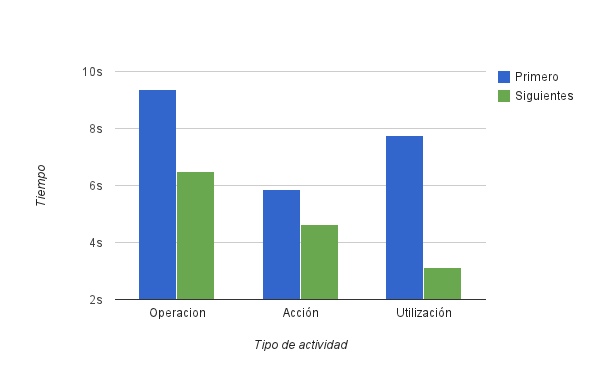
\includegraphics[width=14cm]{resultados/imagenes/interfaz_tiempo_actividades.png}
\caption{Tiempo por tipo de actividad}
\label{fig:interfaz_tiempo_acciones}
\end{figure}

En la figura~\ref{fig:interfaz_tiempo_acciones} se observa como en promedio el
usuario aprende, y en las siguientes acciones similares demora menos tiempo,
este es un factor importante y es el objetivo de esta prueba pues muestra que la
interfaz es fácil de usar, y con tres movimientos básicos, el usuario puede
utilizarla sin mayores inconvenientes. Se observa una mejoría del $30\%$ en las
acciones \emph{Menú Contextual}, $21\%$ en las acciones de tipo \emph{Menú de la
    Interfaz} y finalmente, una mejoría del $60\%$ en las acciones de tipo
\emph{Herramienta}.


La tabla~\ref{tab:interfaz_cantidad_espaciales} nos muestra la cantidad de
movimientos espaciales realizados por los usuarios, se observa que en promedio
se desplazaron $10,88$ veces por el escenario, y $6,75$ veces acercaron o
alejaron la cámara del paciente.

\observacion{Hay que dejar bien en claro de donde sale esto, por que es
importante entender el significado de esta diferencia}

\begin{table}[H]
\centering
\begin{tabular}{lrrr}
\toprule
\textbf{Jugador}  & \textbf{Movimiento} & \textbf{Zoom} & \textbf{Total} \\
\midrule
1        & 18         & 2    & 20 \\
2        & 7          & 8    & 15 \\
3        & 14         & 12   & 26 \\
4        & 9          & 14   & 23 \\
5        & 5          & 8    & 13 \\
6        & 14         & 4    & 18 \\
7        & 16         & 3    & 19 \\
8        & 4          & 3    &  7 \\
\midrule
\textbf{Promedio} & \textbf{10,88}      & \textbf{6,75} & \textbf{17,63} \\
\bottomrule
\end{tabular}
\caption{Cantidad de movimientos espaciales}
\label{tab:interfaz_cantidad_espaciales}
\end{table}

No existe una cantidad mínima o máxima que el usuario debería acercar o mover la
cámara, en cambio, los datos mostrados en~\ref{tab:interfaz_cantidad_espaciales},
muestran que no son necesarias demasiadas acciones, juntando esta información,
con la información proveída en la tabla~\ref{tab:interfaz_tiempo_total}, se ve
que en promedio los usuarios realizaron $1,7$ movimientos por minuto.

\begin{table}[!hbt]
\centering
\begin{tabular}{lrrr}
\toprule
\textbf{Alumno} & \textbf{Tiempo} \\
\midrule
1        & 8:32 \\
2        & 6:03 \\
3        & 8:33 \\
4        & 5:17 \\
5        & 6:55 \\
6        & 8:40 \\
7        & 7:03 \\
8        & 10:27 \\
\midrule
\textbf{Promedio} & \textbf{7:41} \\
\bottomrule
\end{tabular}
\caption{Tiempo de prueba por usuario}
\label{tab:interfaz_tiempo_total}
\end{table}

El tiempo total que se observa en la tabla~\ref{tab:interfaz_tiempo_total},
muestra que en promedio a cada alumno le tomo $7:41$ minutos realizar todos los
pasos especificados, es importante notar que este tiempo incluye el tiempo de
adaptación. 



\begin{table}[!hbt]
\centering
\begin{tabular}{lrrr}
\toprule
\textbf{Alumno} & \textbf{Pasos requeridos} \\
\midrule
1 & 19 \\
2 & 15 \\
3 & 18 \\
4 & 15 \\
5 & 18 \\
6 & 16 \\
7 & 19 \\
8 & 14 \\
\midrule
\textbf{Promedio} & \textbf{16,75} \\
\bottomrule
\end{tabular}
\caption{Acciones realizadas por usuario}
\label{tab:interfaz_acciones}
\end{table}

La tabla~\ref{tab:interfaz_acciones} nos muestra la cantidad de acciones que
realizaron los alumnos, junto con las acciones correctas para llevar a cabo el
procedimiento. Se observa que en promedio realizaron $16.75$ acciones correctas,
esto permite identificar en que parte de procedimiento los usuarios tienen
inconvenientes en cuanto al uso de la interfaz.

\subsection{Resultados de la encuesta}
\label{sec:res_interfaz}

\fixme{Como fue descripta en la sección~\ref{sec:interfaz} la encuesta es
realizada a cada usuario}{Mejorar}, y es utilizada para obtener el grado de
disconformidad de los mismos. Se utiliza la disconformidad para resaltar los
puntos débiles, y así, aquellas variables que tengan el mayor porcentaje serán
las que deben ser arregladas.

Las preguntas que forman parte de la  encuesta son agrupadas en cuanto a
aspectos de calidad gráfica, interacción con el entorno, interacción con los
objetos, características del entorno, usabilidad de la interfaz e integración
con el hardware.

Luego de estas agrupaciones obtenemos el resultado que se muestra en la
tabla~\ref{tab:interfaz_disconformidad_metrica}. En esta tabla se puede observar
que las mayores disconformidades son con respecto a la usabilidad de la interfaz
que llega al $51\%$, la interacción de los usuarios con el entorno que llega al
$50\%$, la interacción con los objetos que llega al $49\%$. Luego, se pueden
observar también otras disconformidades con menor porcentaje, las
características del entorno con un  $33\%$, la integración con el hardware con
un  $27\%$ y por ultimo, la calidad gráfica con un  $17\%$.

\observacion{Hay que explicar que estas pruebas se hicieron de forma previa a
las demás y que se arreglan algunos casos}

\begin{table}[H]
\centering
\begin{tabular}{lr}
\toprule
Métrica & Disconformidad \\
\midrule
Calidad Gráfica         & 0.17 \\
Interacción Entorno     & 0.50\\
Interacción Objetos     & 0.49\\
Características Entorno & 0.33\\
Usabililidad Interfaz   & 0.51\\
Integración Hardware    & 0.27\\
\bottomrule
\end{tabular}
\caption{Disconformidad por métrica}
\label{tab:interfaz_disconformidad_metrica}
\end{table}

La conclusión de esta prueba de interfaz, es que si bien, pudo ser utilizada sin
mayores inconvenientes, existe un alto grado de disconformidad con la interfaz,
además cabe resaltar, los sujetos de prueba son personas acostumbradas al uso de
tecnologías similares. Otros puntos débiles encontrados en esta prueba son la
interacción con el entorno y  con los objetos.

Como resultado de esta prueba, la interfaz y la interacción con objetos y
elementos sufren modificaciones a fin de su utilización con usuarios no
técnicos.

Las demás pruebas mencionadas en este capítulo son realizadas con la versión
final de la solución, la cual es obtenida luego de las mejoras realizadas a los
puntos débiles detectados por esta prueba.
